\section{Definition des Szenarioumfelds}
\label{environment}

Gegenstand des folgenden Kapitels soll es sein, relevante Umweltfaktoren herauszuheben. Dies geschieht  im Branchen- sowie im Technologiekontext des Untersuchungsobjekt Cloud Computing. 

\subsection{Branchenumfeld}
Die Skola GmbH bewegt sich im Umfeld der deutschen Bildungsbranche. Diese Eingrenzung ist wichtig zu erwähnen, da dass deutsche Bildungswesen durch seine förderalen Strukturen einige Probleme mit sich bringt \cite{grella}. Zwar vertreibt das Unternehmen aus diesem Grund in den verschiedenen Bundesländern andere Auflagen von Schulbüchern, auf den Einsatz des Cloud Computing hat dies aber nur geringfügig Einfluss. Lediglich aufgrund der verschiedenen Datenschutzbestimmungen aller Bundesländer sollte eine differenzierte Betrachtung der Umfeldeinflüsse eingegangen werden. Dies ist aber nicht Gegenstand der vorliegenden Arbeit. Die im Abschnitt \ref{conclusion} erstellten Handlungsempfehlungen zielen auf den allgemeinen Einsatz für das Unternehmen und lassen sich sogar global ausdehnen.

Im Umfeld der deutschen Schulbuchverlage breitet sich zum gegenwärtigen Zeitpunkt ein regelrechter \textit{Hype} im Einsatz von mobilen Lernapplikationen aus \cite{specht}. Bücher und Arbeitsmaterialien werden zunehmend webbasiert angeboten. In diesem Kontext spielen Cloud Technologien eine sehr wichtige Rolle. Die Skola GmbH versäumte es mit dem derzeit einseitigen Offline-Angebot von Lehrbüchern in diese Entwicklung einzusteigen. Der Konkurrenzdruck ist demzufolge enorm.
	
\subsection{Technologieumfeld}
Wie bereits mehrfach erläutert ist das Technologiefeld \textit{Cloud Computing} das zentrale Thema der vorliegenden Arbeit. Folgende Definition ist hierbei hilfreich, um die Wesenszüge der Technologie zu nennen: "Cloud Computing ist ein auf Virtualisierung basierendes IT-Bereitstellungsmodell, bei dem Ressourcen sowohl in Form von Infrastruktur als auch Anwendungen und Daten als verteilter Service über das Internet durch einen oder mehrere Leistungserbringer bereitgestellt werden. Diese Services sind nach Bedarf flexibel skalierbar und können verbrauchsabhängig abgerechnet werden"\footnote{Krcmar et al. (2016) \cite{krcmar}, S. 18}. Man erkennt hier sehr schnell eine Reihe von Vorteilen durch die Verlagerung von Rechenleistung und Diensten in das \textit{World Wide Web}. Abbildung \ref{fig:bigpicture} stellt zu diesem Technologiekomplex eine Übersicht als sogenanntes \textit{Big Picture}.

\begin{figure}
	\centering
	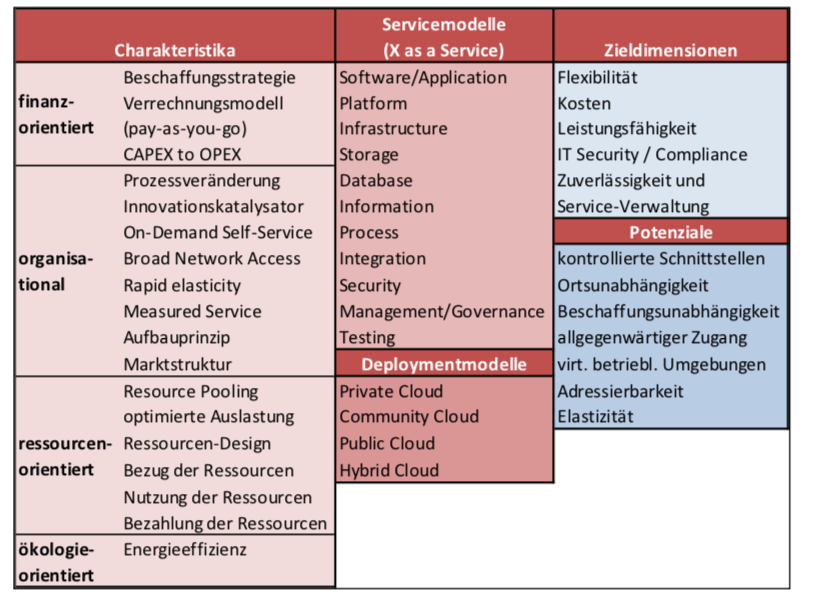
\includegraphics[width=\linewidth]{images/bigpicture}
	\caption[Caption for parameters]{ "Big Picture'' des Cloud Computing nach Stieninger \cite{stieninger}}
	\label{fig:bigpicture}
\end{figure}

Interessant für die spätere Szenariokonstruktion (vgl. Abschnitt \ref{constructions}) sind besonders die verschiedenen Einsatzvarianten. Die Arbeit von Mew hat erwiesen, dass der Einsatz der unterschiedlichen Modelle im Bildungssektor sehr stark gestiegen ist \cite{mew}. Man unterscheidet dabei einerseits in der Bereitstellung und der Art der angebotenen Dienste. Ersteres gliedert sich in folgende Modelle\footnote{Vgl. Stieninger (2013) \cite{stieninger}, S. 14; Baun (2011) \cite{baun}, S. 27}:
\begin{itemize}
	\item \textit{Private Cloud}: Die Infrastruktur/ der Dienst wird explizit für einen einzelnen Kunden zu speziellen Konditionen angeboten.
	\item \textit{Community Cloud}: Die Infrastruktur/ der Dienst wird explizit für einen einzelne Kundengruppe zu speziellen Konditionen angeboten.
	\item \textit{Public Cloud}: Der \textit{Cloud Provider} stellt die Infrastruktur/ den Dienst der breiten Öffentlichkeit zu allgemeinen Konditionen zur Verfügung.
	\item \textit{Hybrid Cloud}: Dies kennzeichnet eine Mischung von mehreren Modellen, die unabhängig voneinander angeboten, aber miteinander verknüpft werden können.
\end{itemize}

Die Art der angebotenen Dienste kann wieder variieren und wird in folgende Modelle untergliedert\footnote{Vgl. Stieninger (2013) \cite{stieninger}, S. 13f.; Baun (2011) \cite{baun}, S. 31-39.}:
\begin{itemize}
	\item \textit{Software as a Service (SaaS)}: Dem Kunden werden Softwareanwendungen zur Verfügung gestellt.
	\item \textit{Platform as a Service (PaaS)}: Dem Kunden werden (nur) grundsätzliche Infrastrukturen, wie z.B. Betriebssysteme, zur Verfügung gestellt
	\item \textit{Infrastructure as a Service (IaaS)}: Dem Kunden wird die komplette IT-Infrastruktur zur Verfügung gestellt, wie z.B. Speicherplatz, Anwendungen, Betriebssysteme, Prozessoren usw.
\end{itemize}

Die genannten Modelle können sich je nach Literatur und Anwendungsgebiet unterscheiden. Es gibt zudem noch untergeordnete Modelle, die bestimmte Facetten unterschiedlicher Softwareanwendungen stärker hervorheben. Nachfolgend sind jedoch die aufgeführten Modelle bindend und werden in den Szenarien (vgl. Abschnitt \ref{constructions}) wieder aufgegriffen.